% Soubory musí být v kódování, které je nastaveno v příkazu \usepackage[...]{inputenc}

\documentclass[%        Základní nastavení
%  draft,    				  % Testovací překlad
  12pt,       				% Velikost základního písma je 12 bodů
  a4paper,    				% Formát papíru je A4
  oneside,      			% Jednostranný tisk
%twoside,      			% Dvoustranný tisk (kapitoly a další důležité části tedy začínají na lichých stranách)
  unicode,						% Záložky a metainformace ve výsledném  PDF budou v kódování unicode
]{report}				    	% Dokument třídy 'zpráva', vhodná pro sazbu závěrečných prací s kapitolami

\usepackage[utf8]		  %	Kódování zdrojových souborů je UTF-8
	{inputenc}					% Balíček pro nastavení kódování zdrojových souborů

\usepackage[				% Nastavení geometrie stránky
	bindingoffset=10mm,		% Hřbet pro vazbu
	hmargin={25mm,25mm},	% Vnitřní a vnější okraj
	vmargin={25mm,34mm},	% Horní a dolní okraj
	footskip=17mm,			  % Velikost zápatí
	nohead,					      % Bez záhlaví
	marginparsep=2mm,		  % Vzdálenost marginálií
	marginparwidth=18mm,	% Šířka marginálií
]{geometry}

\usepackage{sectsty}
	%přetypuje nadpisy všech úrovní na bezpatkové, kromě \chapter, která je přenastavena zvlášť v thesis.sty
	\allsectionsfont{\sffamily}

\usepackage{graphicx} % Balíček 'graphicx' pro vkládání obrázků
											% Nutné pro vložení logotypů školy a fakulty

\usepackage[          % Balíček 'acronym' pro sazby zkratek a symbolů
	nohyperlinks				% Nebudou tvořeny hypertextové odkazy do seznamu zkratek
]{acronym}						
											% Nutné pro použití prostředí 'acronym' balíčku 'thesis'

\usepackage[
	breaklinks=true,		% Hypertextové odkazy mohou obsahovat zalomení řádku
	hypertexnames=false % Názvy hypertext. odkazů budou tvořeny nezávisle na názvech TeXu
]{hyperref}						% Balíček 'hyperref' pro sazbu hypertextových odkazů
											% Nutné pro použití příkazu 'pdfsettings' balíčku 'thesis'

\usepackage{pdfpages} % Balíček umožňující vkládat stránky z PDF souborů
                      % Nutné při vkládání titulních listů a zadání přímo
                      % ve formátu PDF z informačního systému

\usepackage{enumitem} % Balíček pro nastavení mezerování v odrážkách
  \setlist{topsep=0pt,partopsep=0pt,noitemsep} % konkrétní nastavení

\usepackage{cmap} 		% Balíček cmap zajišťuje, že PDF vytvořené `pdflatexem' je
											% plně "prohledávatelné" a "kopírovatelné"

%\usepackage{upgreek}	% Balíček pro sazbu stojatých řeckých písmem
											%% např. stojaté pí: \uppi
											%% např. stojaté mí: \upmu (použitelné třeba v mikrometrech)
											%% pozor, grafická nekompatibilita s fonty typu Computer Modern!
                      
%\usepackage{amsmath} %balíček pro sabu náročnější matematiky                 

\usepackage{dirtree}	% sazba adresářové struktury
                      % vhodné pro prezentaci obsahu elektronické přílohy (např. CD)

\usepackage[formats]{listings}	% Balíček pro sazbu zdrojových textů
\lstset{              % nastavení
%	Definice jazyka použitého ve výpisech
%    language=[LaTeX]{TeX},	% LaTeX
%	language={Matlab},		% Matlab
	language={C},           % jazyk C
    basicstyle=\ttfamily,	% definice základního stylu písma
    tabsize=2,			% definice velikosti tabulátoru
    inputencoding=utf8,         % pro soubory uložené v kódování UTF-8
		columns=fixed,  %fixed nebo flexible,
		fontadjust=true %licovani sloupcu
    extendedchars=true,
    literate=%  definice symbolů s diakritikou
    {á}{{\'a}}1
    {č}{{\v{c}}}1
    {ď}{{\v{d}}}1
    {é}{{\'e}}1
    {ě}{{\v{e}}}1
    {í}{{\'i}}1
    {ň}{{\v{n}}}1
    {ó}{{\'o}}1
    {ř}{{\v{r}}}1
    {š}{{\v{s}}}1
    {ť}{{\v{t}}}1
    {ú}{{\'u}}1
    {ů}{{\r{u}}}1
    {ý}{{\'y}}1
    {ž}{{\v{z}}}1
    {Á}{{\'A}}1
    {Č}{{\v{C}}}1
    {Ď}{{\v{D}}}1
    {É}{{\'E}}1
    {Ě}{{\v{E}}}1
    {Í}{{\'I}}1
    {Ň}{{\v{N}}}1
    {Ó}{{\'O}}1
    {Ř}{{\v{R}}}1
    {Š}{{\v{S}}}1
    {Ť}{{\v{T}}}1
    {Ú}{{\'U}}1
    {Ů}{{\r{U}}}1
    {Ý}{{\'Y}}1
    {Ž}{{\v{Z}}}1
}

%%%%%%%%%%%%%%%%%%%%%%%%%%%%%%%%%%%%%%%%%%%%%%%%%%%%%%%%%%%%%%%%%
%%%%%%      Definice informací o dokumentu             %%%%%%%%%%
%%%%%%%%%%%%%%%%%%%%%%%%%%%%%%%%%%%%%%%%%%%%%%%%%%%%%%%%%%%%%%%%%

% V tomto souboru se nastavují téměř veškeré informace, proměnné mezi studenty:
% jméno, název práce, pohlaví atd.
% Tento soubor je SDÍLENÝ mezi textem práce a prezentací k obhajobě -- netřeba něco nastavovat na dvou místech.

\usepackage[
%%% Z následujících voleb jazyka lze použít pouze jednu
  czech-english,		% originální jazyk je čeština, překlad je anglicky (výchozí)
  %english-czech,	% originální jazyk je angličtina, překlad je česky
  %slovak-english,	% originální jazyk je slovenština, překlad je anglicky
  %english-slovak,	% originální jazyk je angličtina, překlad je slovensky
%
%%% Z následujících voleb typu práce lze použít pouze jednu
  %semestral,		  % semestrální práce (nesází se abstrakty, prohlášení, poděkování) (výchozí)
  %bachelor,			%	bakalářská práce
  master,			  % diplomová práce
  %treatise,			% pojednání o disertační práci
  %doctoral,			% disertační práce
%
%%% Z následujících voleb zarovnání objektů lze použít pouze jednu
%  left,				  % rovnice a popisky plovoucích objektů budou zarovnány vlevo
	center,			    % rovnice a popisky plovoucích objektů budou zarovnány na střed (vychozi)
%
]{thesis}   % Balíček pro sazbu studentských prací


%%% Jméno a příjmení autora ve tvaru
%  [tituly před jménem]{Křestní}{Příjmení}[tituly za jménem]
% Pokud osoba nemá titul před/za jménem, smažte celý řetězec '[...]'
\author[Bc.]{David}{Lindtner}

%%% Identifikační číslo autora (VUT ID)
\butid{196815}

%%% Pohlaví autora/autorky
% (nepoužije se ve variantě english-czech ani english-slovak)
% Číselná hodnota: 1...žena, 0...muž
\gender{0}

%%% Jméno a příjmení vedoucího/školitele včetně titulů
%  [tituly před jménem]{Křestní}{Příjmení}[tituly za jménem]
% Pokud osoba nemá titul před/za jménem, smažte celý řetězec '[...]'
\advisor[Ing.]{Petr}{Gábrlík}[Ph.D.]

%%% Jméno a příjmení oponenta včetně titulů
%  [tituly před jménem]{Křestní}{Příjmení}[tituly za jménem]
% Pokud osoba nemá titul před/za jménem, smažte celý řetězec '[...]'
% Nastavení oponenta se uplatní pouze v prezentaci k obhajobě;
% v případě, že nechcete, aby se na titulním snímku prezentace zobrazoval oponent, pouze příkaz zakomentujte;
% u obhajoby semestrální práce se oponent nezobrazuje (jelikož neexistuje)
% U dizertační práce jsou typicky dva až tři oponenti. Pokud je chcete mít na titulním slajdu, prosím ručně odkomentujte a upravte jejich jména v definici "VUT title page" v souboru thesis.sty.
\opponent[doc.\ Mgr.]{Křestní}{Příjmení}[Ph.D.]

%%% Název práce
%  Parametr ve složených závorkách {} je název v originálním jazyce,
%  parametr v hranatých závorkách [] je překlad (podle toho jaký je originální jazyk).
%  V případě, že název Vaší práce je dlouhý a nevleze se celý do zápatí prezentace, použijte příkaz
%  \def\insertshorttitle{Zkác.\ náz.\ práce}
%  kde jako parametr vyplníte zkrácený název. Pokud nechcete zkracovat název, budete muset předefinovat,
%  jak se vytváří patička slidu. Viz odkaz: https://bit.ly/3EJTp5A
\title[Simulation of Unmanned Aircrafts in a Virtual Environment]{Simulace bezpilotních letadel ve virtuálním prostředí}

%%% Označení oboru studia
%  Parametr ve složených závorkách {} je název oboru v originálním jazyce,
%  parametr v hranatých závorkách [] je překlad
\specialization[Cybernetics, Control and Measurements]{Kybernetika, automatizace a měření}

%%% Označení ústavu
%  Parametr ve složených závorkách {} je název ústavu v originálním jazyce,
%  parametr v hranatých závorkách [] je překlad
\department[Department of Control and Instrumentation]{Ústav automatizace a měřicí techniky}
%\department[Department of Biomedical Engineering]{Ústav biomedicínského inženýrství}
%\department[Department of Electrical Power Engineering]{Ústav elektroenergetiky}
%\department[Department of Electrical and Electronic Technology]{Ústav elektrotechnologie}
%\department[Department of Physics]{Ústav fyziky}
%\department[Department of Foreign Languages]{Ústav jazyků}
%\department[Department of Mathematics]{Ústav matematiky}
%\department[Department of Microelectronics]{Ústav mikroelektroniky}
%\department[Department of Radio Electronics]{Ústav radioelektroniky}
%\department[Department of Theoretical and Experimental Electrical Engineering]{Ústav teoretické a experimentální elektrotechniky}
%\department[Department of Telecommunications]{Ústav telekomunikací}
%\department[Department of Power Electrical and Electronic Engineering]{Ústav výkonové elektrotechniky a elektroniky}

%%% Označení fakulty
%  Parametr ve složených závorkách {} je název fakulty v originálním jazyce,
%  parametr v hranatých závorkách [] je překlad
%\faculty[Faculty of Architecture]{Fakulta architektury}
\faculty[Faculty of Electrical Engineering and~Communication]{Fakulta elektrotechniky a~komunikačních technologií}
%\faculty[Faculty of Chemistry]{Fakulta chemická}
%\faculty[Faculty of Information Technology]{Fakulta informačních technologií}
%\faculty[Faculty of Business and Management]{Fakulta podnikatelská}
%\faculty[Faculty of Civil Engineering]{Fakulta stavební}
%\faculty[Faculty of Mechanical Engineering]{Fakulta strojního inženýrství}
%\faculty[Faculty of Fine Arts]{Fakulta výtvarných umění}
%
%Nastavení logotypu (v hranatych zavorkach zkracene logo, ve slozenych plne):
\facultylogo[logo/FEKT_zkratka_barevne_PANTONE_CZ]{logo/UTKO_color_PANTONE_CZ}

%%% Rok odevzdání práce
\graduateyear{2022}
%%% Akademický rok odevzdání práce
\academicyear{2021/22}

%%% Datum obhajoby (uplatní se pouze v prezentaci k obhajobě)
\date{11.\,11.\,1980} 

%%% Místo obhajoby
% Na titulních stránkách bude automaticky vysázeno VELKÝMI písmeny (pokud tyto stránky sází šablona)
\city{Brno}

%%% Abstrakt
\abstract
[The master thesis deals with the issue of simulation of unmanned aircraft missions in~a~virtual environment. The aim of the work is to demonstrate basic and more advanced autonomous aerial missions in the simulated environment Gazebo - ROS 2. The work emphasizes the stability of the software solution and the stability of the communication between critical components of the aerial mission.
]{%
Diplomová práce se zabývá problematikou simulace misí bezpilotních letadel ve virtuálním prostředí. Cílem práce je demonstrovat základní i pokročilejší autonomní letecké mise v~simulovaném prostředí Gazebo - ROS 2. Důraz práce je kladen na stabilitu softwarového řešení a stabilitu komunikace mezi kritickými komponenty letecké mise.
}

%%% Klíčová slova
\keywrds[%
Autonomous mission, Robotics, Drone, Pixhawk, PX4, Autopilot uORB, DDS, RTPS, MAVlink, Mavros, ROS 2, Gazebo, Simulation
]{%
Autonomní mise, Robotika, Dron, Pixhawk, PX4, Autopilot, uORB, DDS, RTPS, MAVLink, Mavros ROS 2, Gazebo, Simulace
}

%%% Poděkování
\acknowledgement{%
Rád bych poděkoval vedoucímu diplomové práce panu Ing.~Petrovi Gabrlíkovi, Ph.D.\ za~odborné vedení, trpělivost, čas strávený na konzultacích a podnětné návrhy k~práci. Dále bych rád poděkoval Bc. Milošovi Cihlářovi za~poskytnutí dat k sestavení simulačního modelu okolí naší školy, které byli výsledkem jeho diplomové práce.
}%
  % do tohoto souboru doplňte údaje o sobě, druhu práce, názvu...

%%%%%%%%%%%%%%%%%%%%%%%%%%%%%%%%%%%%%%%%%%%%%%%%%%%%%%%%%%%%%%%%%%%%%%%%

%%%%%%%%%%%%%%%%%%%%%%%%%%%%%%%%%%%%%%%%%%%%%%%%%%%%%%%%%%%%%%%%%%%%%%%%
%%%%%%     Nastavení polí ve Vlastnostech dokumentu PDF      %%%%%%%%%%%
%%%%%%%%%%%%%%%%%%%%%%%%%%%%%%%%%%%%%%%%%%%%%%%%%%%%%%%%%%%%%%%%%%%%%%%%
%% Při načteném balíčku 'hyperref' lze použít příkaz '\pdfsettings':
\pdfsettings
%  Nastavení polí je možné provést také ručně příkazem:
%\hypersetup{
%  pdftitle={Název studentské práce},    	% Pole 'Document Title'
%  pdfauthor={Autor studenstké práce},   	% Pole 'Author'
%  pdfsubject={Typ práce}, 						  	% Pole 'Subject'
%  pdfkeywords={Klíčová slova}           	% Pole 'Keywords'
%}
%%%%%%%%%%%%%%%%%%%%%%%%%%%%%%%%%%%%%%%%%%%%%%%%%%%%%%%%%%%%%%%%%%%%%%%

\pdfmapfile{=vafle.map}

%%%%%%%%%%%%%%%%%%%%%%%%%%%%%%%%%%%%%%%%%%%%%%%%%%%%%%%%%%%%%%%%%%%%%%%
%%%%%%%%%%%       Začátek dokumentu               %%%%%%%%%%%%%%%%%%%%%
%%%%%%%%%%%%%%%%%%%%%%%%%%%%%%%%%%%%%%%%%%%%%%%%%%%%%%%%%%%%%%%%%%%%%%%
\begin{document}
\pagestyle{empty} %vypnutí číslování stránek

%% Vložení desek 
\includepdf[pages=1]%  buďto generovaných informačním systémem
  {pdf/desky}% název souboru nesmí obsahovat mezery!
%% NEBO vytvoření desek z balíčku
%\makecover
%%
%\oddpage % při dvojstranném tisku přidá prázdnou stránku
% kazdopádně ale:
\setcounter{page}{1} %resetovaní čítače stránek -- desky do číslování nezahrnujeme

%% Vložení titulního listu
\includepdf[pages=1]%    buďto generovaného informačním systémem
  {pdf/TitulniList_color}% název souboru nesmí obsahovat mezery!
%% NEBO vytvoření titulní stránky z balíčku
%\maketitle
%%
%\oddpage  % při dvojstranném tisku se přidá prázdná stránka
   
%% Vložení zadání
\includepdf[pages=1]%   buďto generovaného informačním systémem
  {pdf/zadani}% název souboru nesmí obsahovat mezery!
%% NEBO lze vytvořit prázdný list příkazem ze šablony
%\patternpage{}%
%	{\sffamily\Huge\centering ZDE VLOŽIT LIST ZADÁNÍ}%
%	{\sffamily\centering Z~důvodu správného číslování stránek}
%%
%\oddpage% při dvojstranném tisku se přidá prázdná stránka

%% Vysázení stránky s abstraktem
\makeabstract

% Vysázení stránky s rozšířeným abstraktem
% (pokud píšete práci v češtině či slovenštině, vložení rozšířeného abstraktu zrušte;
%  pro semestrální projekt také není potřeba rozšířený abstrakt uvádět)
%\input{text/rozsireny_abstrakt}

%%% Vysázení citace práce
\makecitation

%%% Vysázení prohlášení o samostatnosti
\makedeclaration

%%% Vysázení poděkování
\makeacknowledgement

%%% Vysázení obsahu
\tableofcontents

%%% Vysázení seznamu obrázků
% (vynechejte, pokud máte dva nebo méně obrázků)
\listoffigures

%%% Vysázení seznamu tabulek
% (vynechejte, pokud máte dvě nebo méně tabulek)
\listoftables

%%% Vysázení seznamu výpisů kódu
% (vynechejte, pokud máte dva nebo méně výpisů)
\lstlistoflistings

\cleardoublepage\pagestyle{plain}   % zapnutí číslování stránek

%Pro vkládání kapitol i příloh používejte raději \include než \input
%%% Vložení souboru 'text/uvod.tex' s úvodem
\chapter*{Úvod}
\phantomsection
\addcontentsline{toc}{chapter}{Úvod}

DOKONČIŤ

Téma bezpilotních letadel a autonomních leteckých misí v poslední době nabývá na popularitě. S drony se začínáme setkávat v běžném životě, ale také v dalších odvětvích jako jsou armáda, lesnictví, zemědělství a stavitelství. Simulace je vhodným přístupem k vývoji autonomních letadel, protože snižuje finanční nároky a urychluje vývoj a testování.

Tato práce se bude zabývat problematikou simulace misí bezpilotních letadel ve virtuálním prostředí. Cílem práce je seznámit se s simulačním ekosystémem Gazebo/ROS2 a vytvořit a demonstrovat jednoduchou autonomní misi.

Práce bude pojednávat o topologii řídícího systému dronu, jak ze stránky nízkoúrovňového řízení, tak z pohledu palubního počítače pro řízení složitých autonomních misí.

V práci bude popsaný firmware řídící jednotky, možnosti nastavení parametrů letu dronu, možnosti komunikace s okolím a hlavně komunikace s ROS 2.

Práce se věnuje instalaci a nastavení simulačního prostředí. Bude zde přiblížen praktický test simulované autonomní mise v prostředí PX4 - Gazebo, v které dron dostává povely z nadřazeného systému palubního počítače na báze ROS 2.


\chapter{Topologie dronu}

Práce se zaobírá v první řadě simulací bezpilotních letadel ve virtuálním prostředí, ale z důvodu možné budoucí realizace projektu je nutné pracovat s konkrétními hardwarovými a softwarovými řešeními.

Topologii řídícího systému dronu jsme rozdělili na dvě části. Palubní počítač řídí bezplotnou misi a řídící jednotka ovládá kritické procesy v dronu. Na trhu existuje nepřeberné množství různých komponent pro autonomní mise. Na základě existujících projektů, například \textit{Multi Robot Systems Group} z ČVUT \cite{MRS} jsme zvolili modul Pixhawk jako řídící jednotku. Jako palubní počítač, který ovládá samotnou autonomní misi jsme zvolili jednodeskový počítač Raspberry PI.

S touto kombinací jsme schopni řídit velké množství různých autonomních letadel a vozidel jako jsou:

\begin{itemize}
    \item dron v různých konfiguracích
    \item delta \acs{VTOL} (\acl{VTOL})
    \item letadlo v různých konfiguracích
    \item vrtulník
    \item rover
    \item ponorka
\end{itemize}

\section{Řídící jednotka Pixhawk}

Pixhawk je otevřený hardwarový projekt, jehož cílem je poskytnout standard pro snadno dostupné a vysoce kvalitní návrhy hardwaru autopilota pro akademické, hobby a vývojářské komunity. \cite{PIX1}

Řídící jednotka Pixhawk řídí kritické procesy v dronu jako \textit{fail safe} funkce, ovládání pohonů, stabilizace a čtení kritických snímačů (GPS, barometr) pro řízení dronu.

Existuje několik 

\begin{itemize}
    \item Pixhawk (výroba byla ukončena)
    \item Pixhawk 2 (výroba byla ukončena)
    \item Pixhawk 3 Pro
    \item Pixhawk 4
    \item Pixhawk 4 Mini
    \item Pixhawk 5X
    \item Pixracer
    \item Auterion Skynode (průmyslové řešení)
\end{itemize}

\begin{figure}[!ht]
    \begin{center}
        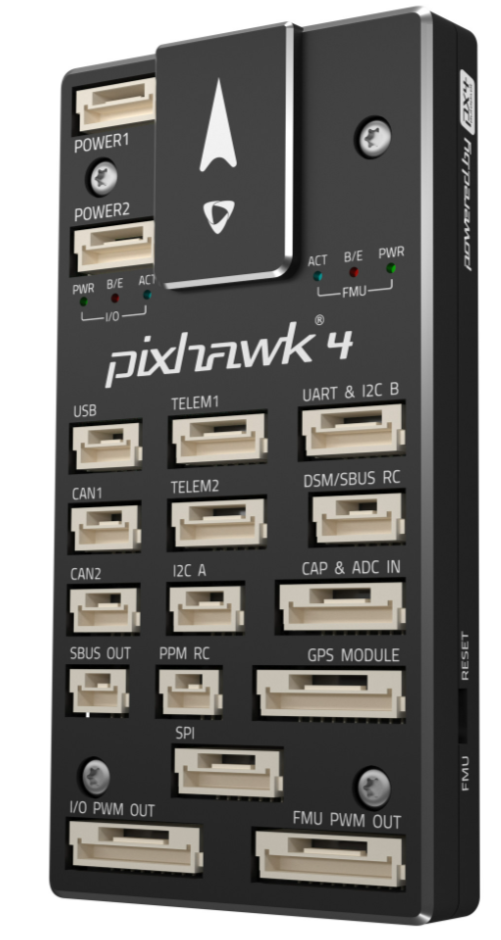
\includegraphics[scale=0.47]{obrazky/PIX}
    \end{center}
    \caption[Řídící jednotka Pixhawk 4]{Řídící jednotka Pixhawk 4 \cite{PIX2}.}
    \label{fig:PIX}
\end{figure}

\section{Palubní počítač}

Jako palubní počítač se pro experimentální letecké mise využívá jednodeskový počítač Raspberry PI. Na trhu existuje množství různých variant tohoto široce rozšířeného počítače v rozmezí od levného, malého a úsporného  \textit{Raspberry PI Pico} až po vysoce výkonný počítač \textit{Raspberry PI 4}.

Důležitými výhodami pro aplikace v robotických misích jsou integrace na jeden plošní spoj, nízká proudová spotřeba a možnost spuštění linuxových distribucí. Nejběžnější podporované distribuce jsou Raspberry PI OS, Raspbian, Ubuntu desktop a server.

Hlavní důvod pro použití Raspberry PI jako palubního počítače je možnost spolehlivé komunikace s PX4 firmware přes ROS 2 \textit{topic}. Komunikací mezi uvedenými platformami se budeme zabývat v následujících kapitolách.
\chapter{Firmware pro řízení bezpilotních letadel}

\section{BetaFlight}

BetaFlight je \textit{open-source} firmware pro řízení letu používaný k létání s multikoptérami a s letadly s pevnými křídly. Firmware se zaměřuje na letový výkon, špičkové funkce a širokou podporu platforem.

BetaFlight podporuje velkou škálu řídících jednotek, které mají alespoň \textit{STM32F4} procesor. Software pro nastavování parametrů (\textit{BetaFlight Configurator}) běží na Windows, Mac OS, Linux a Android.

Firmware Betaflight podporuje komunikaci s dálkovými ovládači od většiny výrobců, jako jsou FrSky, Graupner, Spektrum, DJI a FlySky. Řídící jednotku s BetaFlight firmware je možné povelovat i z nadřazeného systému pomocí \textit{\acs{MSP}} \footnote{\acs{MSP} (\acl{MSP}) je komunikační protokol pro posílání informací o telemetrii, dat ze snímačů a ovládání \cite{ARDU}}. \cite{BetaF}

\section{INAV}

INAV autopilot je odvozený od BetaFlight a zaměřuje se hlavně na autonomní lítání. Podporuje velké množstvi modelů od závodních a freestyle dronů, přez letadla až pod rovery a jiné kolové vozidla.

Firmware podporuje širokou škálu řídících jednotek od různých výrobců, podporuje zpracování dat ze senzorů a umožňuje ukládání dat o letu a vnitřním stavu dronu v reálném čase (\textit{blackbox}). \cite{INAV}

Software\textbf{} \textit{INAV Configurator} nabízí plánování \textit{waypoint} mise pro jakýkoliv autonomní model s řídící jednotkou, v které běží INAV firmware.

\section{Firmware pro řídící jednotku Pixhawk}

Existují dvě hlavní větve vývoje firmware pro řídící jednotku Pixhawk. Jednou platformou je open source projekt ArduPilot \cite{ARDU}, který podporuje velké množství bezpilotních prostředků a umožňuje vytváření autonomních misí. Druhým projektem je profesionální autopilot PX4 \cite{PX4ORG}. Velkou výhodou obou projektů je, že jsou do velké části kompatibilní, například software pro pozemní stanice QGroundControl z platformy PX4 může komunikovat s řídící jednotkou s firmware od ArduPilot a naopak. Vzájemná kompatibilita je zajištěna využitím stejného komunikačního protokolu MAVLink. Výhoda protokolu MAVLink spočívá aj v tom, že oba firmware můžou komunikovat s ROS (Robot Operating System) přes MAVROS\footnote{MAVROS je komunikační ovládač (\textit{driver}) pro komunikaci mezi ROS a autopiloty s MAVLink protokolem}

\subsection{ArduPilot}

ArduPilot je open source autopilot podporující mnoho typů vozidel, například multikoptéry, tradiční vrtulníky, letadla s pevnými křídly, čluny, ponorky, rovery a další. Projekt ArduPilot má společnou historii s PX4, ale v minulosti se tyto dva projekty oddělili. Proto mají oba projekty do velké míry podobné využití a míří na stejnou platformu.

Zdrojový kód projektu ArduPilot je vyvíjen širokým spektrem profesionálů a nadšenců, takže výhodou je velká komunita poskytující řešení na řadu problémů.

Frimware ArduPilot je založený na ChibiOS \acs{RTOS} (\acl{RTOS}). ArduPilot taky poskytuje možnost simulace letového kódu jak simulací \acs{SITL} (\acl{SITL}), tak simulací \acs{HITL} (\acl{HITL}). \cite{ARDU}

Pro další pokračování v práci jsme zvolili projekt PX4, takže další části budou pojednávat o firmware PX4.


\chapter{PX4 autopilot}

PX4 je profesionální autopilot, vyvinutý světovými vývojáři z průmyslu a akademické obce a podporovaný aktivní celosvětovou komunitou. Pohání všechny druhy vozidel od závodních a nákladních dronů až po pozemní vozidla a ponorky. 

\section{Architektura PX4}

PX4 firmware se skládá ze dvou hlavních vrstev:
\begin{itemize}
    \item Flight stack (letový zásobník)
    \begin{itemize}
        \item Letový zásobník je systém pro odhad a řízení letu.
    \end{itemize}
    \item PX4 middleware
    \begin{itemize}
        \item PX4 middleware je obecná robotická vrstva, která podporuje jakýkoli typ autonomního robota a poskytuje interní/externí komunikaci a integraci s hardware.
        \item Middleware navíc obsahuje simulační vrstvu, která umožňuje spuštění letového kódu PX4 na desktopovém operačním systému a ovládání počítačem modelovaného vozidla v simulovaném prostoru.\\
    \end{itemize}
\end{itemize}

Všechny podporované typy vozidel (drony, letadla, čluny, rovery, ponorky atd.) sdílejí jedinou kódovou základnu, která má následující vlastnosti: \cite{PX4main}

\begin{itemize}
    \item Veškerá funkčnost je rozdělena na vyměnitelné a opakovaně použitelné komponenty
    \item Komunikace probíhá pomocí asynchronního předávání zpráv
    \item Systém se dokáže vypořádat s různou pracovní zátěží\\
\end{itemize}

Na obrázku \ref{fig:PX4_Arch} je zobrazen diagram, který poskytuje podrobný přehled stavebních bloků PX4. Horní část diagramu obsahuje middlewarové bloky, zatímco spodní část zobrazuje komponenty letového zásobníku (\textit{flight stack}).

Moduly spolu komunikují prostřednictvím sběrnice \textit{publish-subscribe} s názvem \textit{uORB}. Hlavní výhody schématu \textit{publish-subscribe} v PX4 jsou následující:

\begin{itemize}
    \item Systém je asynchronní a aktualizuje se okamžitě, když jsou k dispozici nová data
    \item Všechny operace a komunikace jsou plně paralelní
    \item Systémová komponenta může zpracovávat data odkudkoli (globální datový prostor)
\end{itemize}

\begin{figure}[!ht]
    \begin{center}
        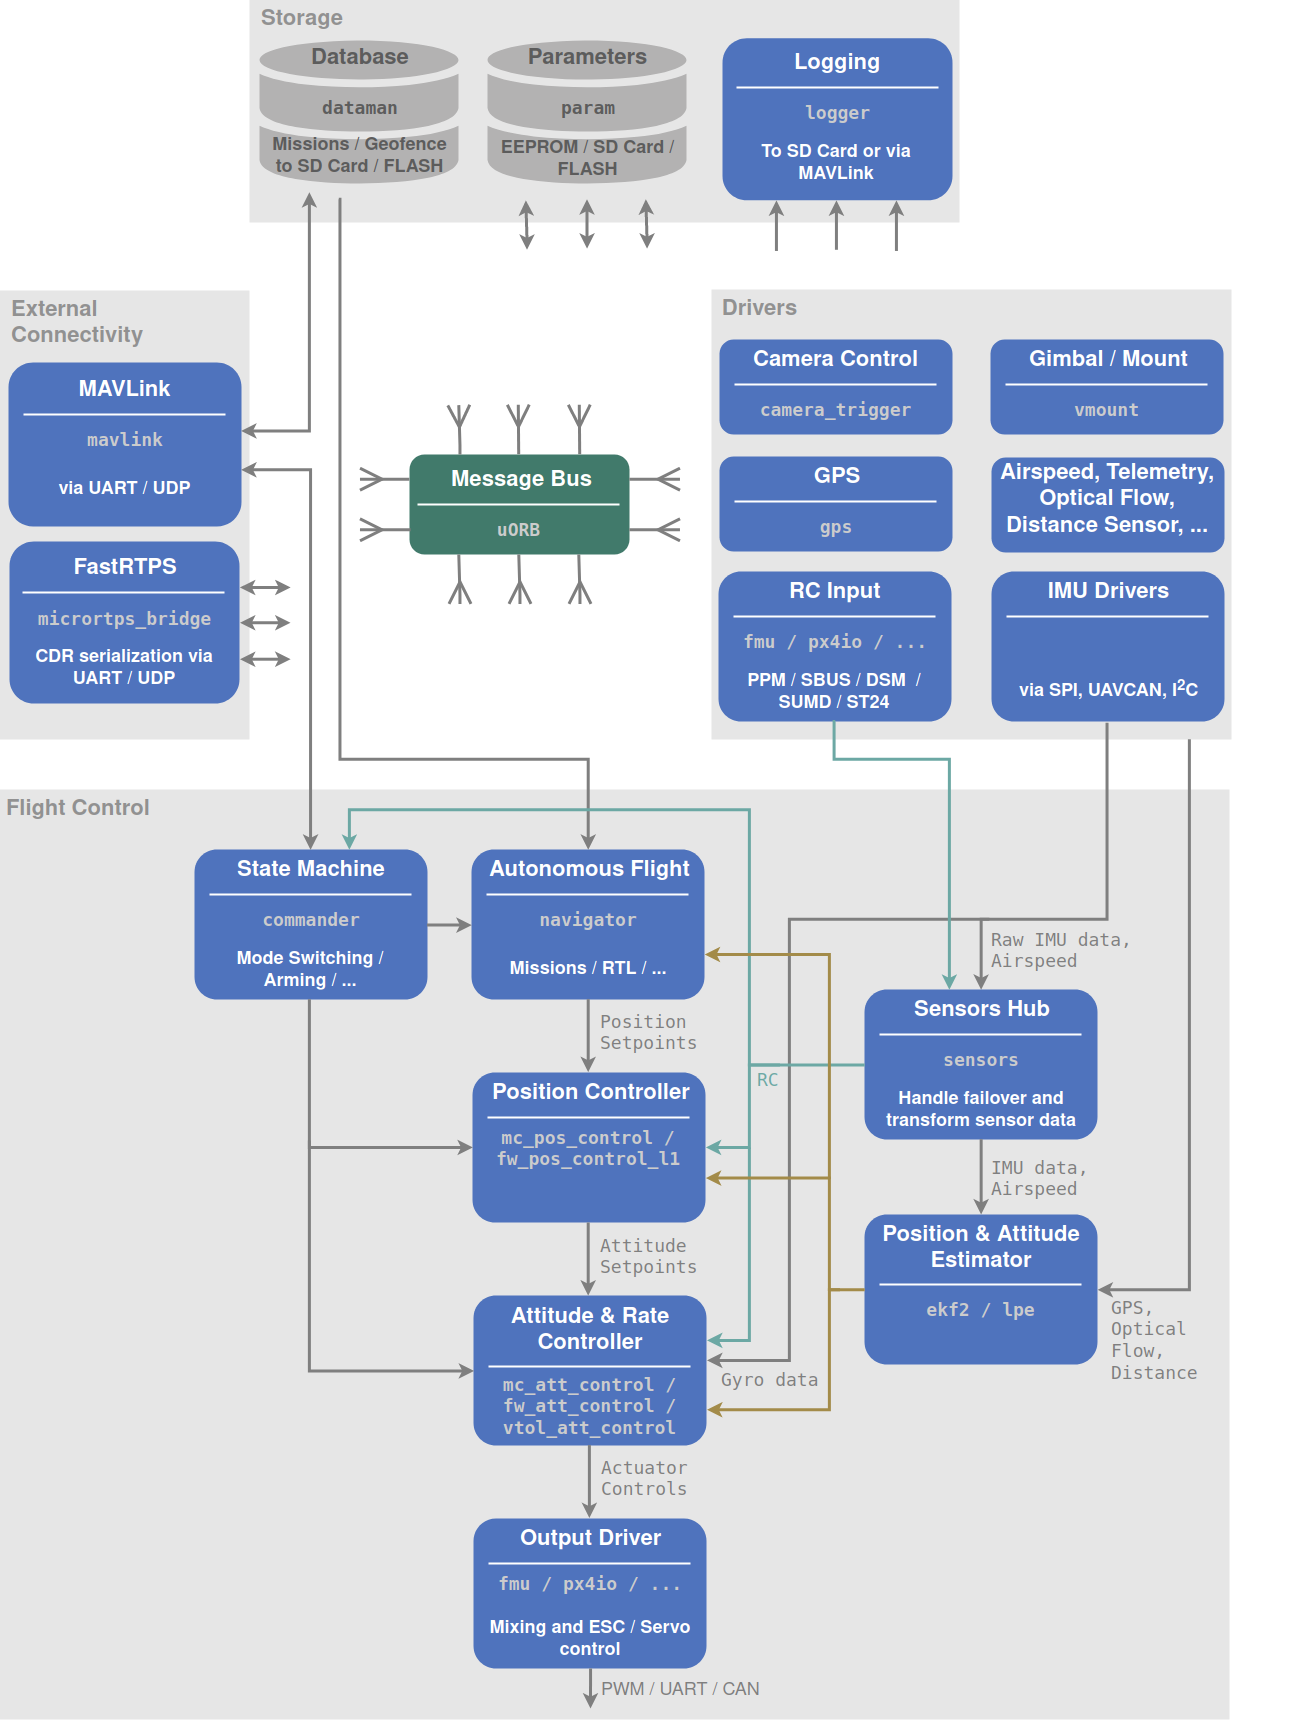
\includegraphics[scale=0.45]{obrazky/PX41}
    \end{center}
    \caption[Komplexní strukturální architektura PX4 software]{Komplexní strukturální architektura PX4 software \cite{PX4main}.}
    \label{fig:PX4_Arch}
\end{figure}

\subsection{PX4 jako samotný letový ovladač}

Na obrázku \ref{fig:PX4_FC} je naznačená architektura systému založeného na letovém ovladači (řídící jednotce) (\textit{flight controller}). Řídící jednotka zabezpečuje sběr dat ze senzorů, ovládání akčních členů dronu (pohony, serva, ...), řízení dronu na základě dat ze senzorů a povelů z RC rádia a v neposlední řadě stabilizaci dronu.

Do systému PX4 je možné zasílat povely z pozemní stanice (\textit{Ground Station}) přes protokol \textit{MAVlink} pomocí telemetrické rádiové soupravy.

\begin{figure}[!ht]
    \begin{center}
        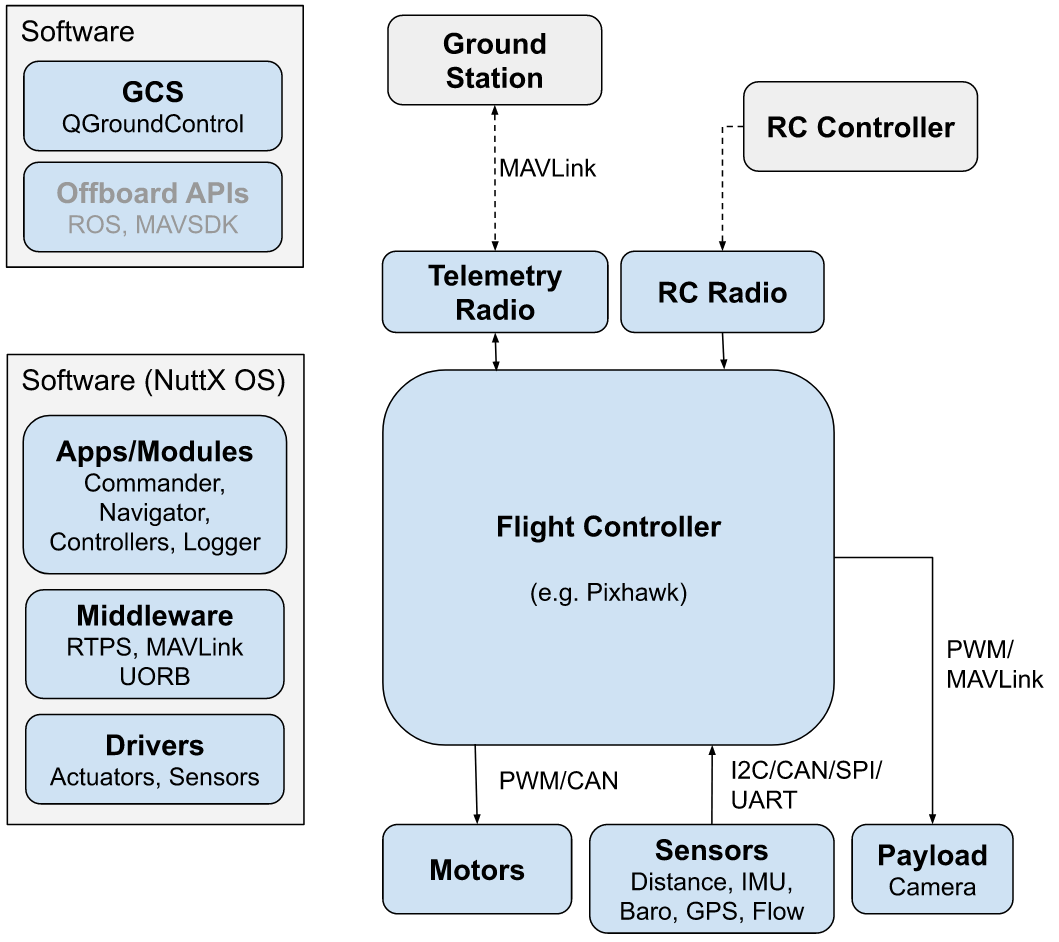
\includegraphics[scale=0.36]{obrazky/PX42}
    \end{center}
    \caption[Jednoduchý systém PX4 založený na letovém ovladači (flight controller)]{Jednoduchý systém PX4 založený na letovém ovladači (flight controller) \cite{PX4main2}.}
    \label{fig:PX4_FC}
\end{figure}

\subsection{Letový ovladač a počítač pro řízení mise}

Na obrázku \ref{fig:PX4_FC_PC} je zobrazená architektura systému PX4 založeného na letovém ovladači (řídící jednotce) a palubním počítači pro řízení mise. Řídící jednotka zabezpečuje sběr dat ze senzorů a ovládání akčních členů dronu (pohony, serva, ...). Komunikace mezi řídící jednotkou zabezpečuje protokol MAVlink, nebo \acs{RTPS} (\acl{RTPS}).

Palubní počítač pro řízení mise poskytuje pokročilé funkce, jako je vyhýbání se objektům a předcházení kolizím. Obvyklým operačním systémem je Linux s ROS (ROS 2) z důvodu, podpory knihoven na předcházení kolizím a z důvodu, že ROS 2 a PX4 využívají pro komunikaci s okolím \acs{DDS} (\acl{DDS}) middleware.

\begin{figure}[!ht]
    \begin{center}
        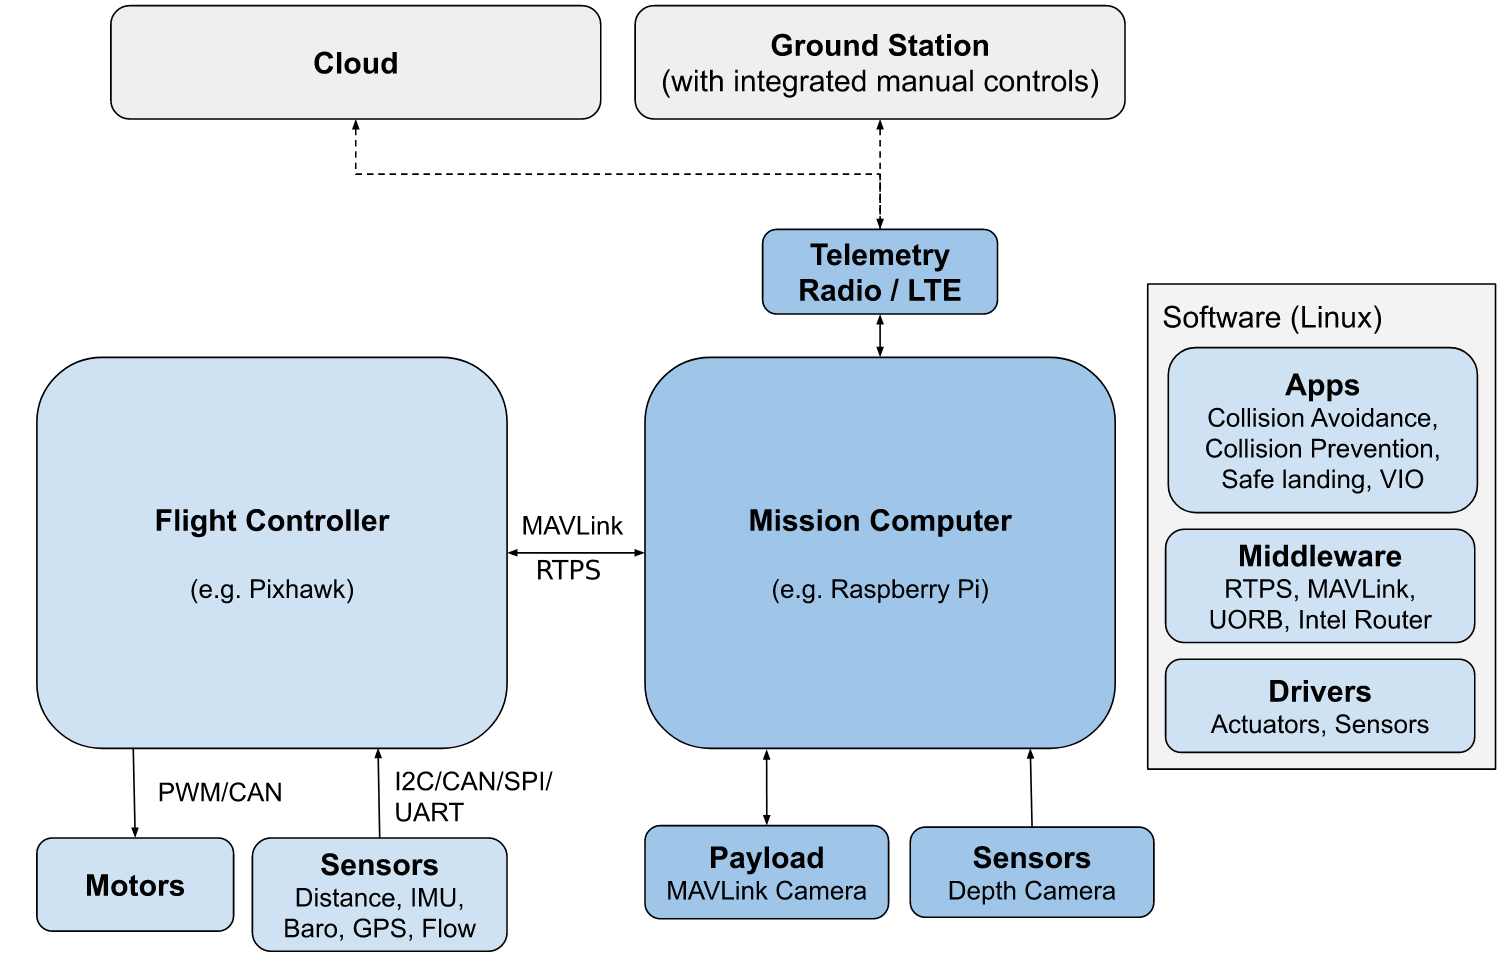
\includegraphics[scale=0.37]{obrazky/PX43}
    \end{center}
    \caption[Systém PX4 založený na letovém ovladači (flight controller) a palubním počítači pro řízení mise]{Systém PX4 založený na letovém ovladači (flight controller) a palubním počítači pro řízení mise \cite{PX4main2}.}
    \label{fig:PX4_FC_PC}
\end{figure}

\section{Licence}

Kód PX4 je zdarma k použití a úpravě za podmínek permisivní licence \textit{BSD 3-clause license} \cite{BSDlicense}.

Redistribuce a použití ve zdrojové a binární formě, s úpravami nebo bez nich, jsou povoleny za předpokladu, že jsou splněny následující podmínky:

1. Redistribuce zdrojového kódu musí obsahovat výše uvedenou poznámku o autorských právech, tento seznam podmínek a následující prohlášení o vyloučení odpovědnosti.

2. Redistribuce v binární formě musí reprodukovat výše uvedenou poznámku o autorských právech, tento seznam podmínek a následující prohlášení o vyloučení odpovědnosti v dokumentaci a/nebo jiných materiálech dodávaných s distribucí.

3. Jméno držitele autorských práv ani jména jeho přispěvatelů nesmí být použita k podpoře nebo propagaci produktů odvozených z tohoto software bez předchozího výslovného písemného povolení.

\section{QGround Control}

QGroundControl je software, který poskytuje plnou kontrolu letu a plánování mise pro jakýkoli dron s podporou MAVLink. Jeho primárním cílem je snadné použití pro profesionální uživatele a vývojáře. Veškerý kód je open source, takže je možné přispívat a dál ho vyvíjet \cite{QGround}.

Pomocí QGroundControl je možné nahrát nejnovější PX4, nebo Ardupilot firmware do letového ovladače (\textit{flight controller}), nastavit typ konstrukce dronu, ladit parametry regulace a vytvářet autonomní mise pomocí waypointů. Veškeré nastavení dronu a misí je jednoduché a velmi intuitivní.

Obrázek \ref{fig:QGC} zobrazuje základní obrazovku software QGroundControl.

\begin{figure}[!ht]
    \begin{center}
        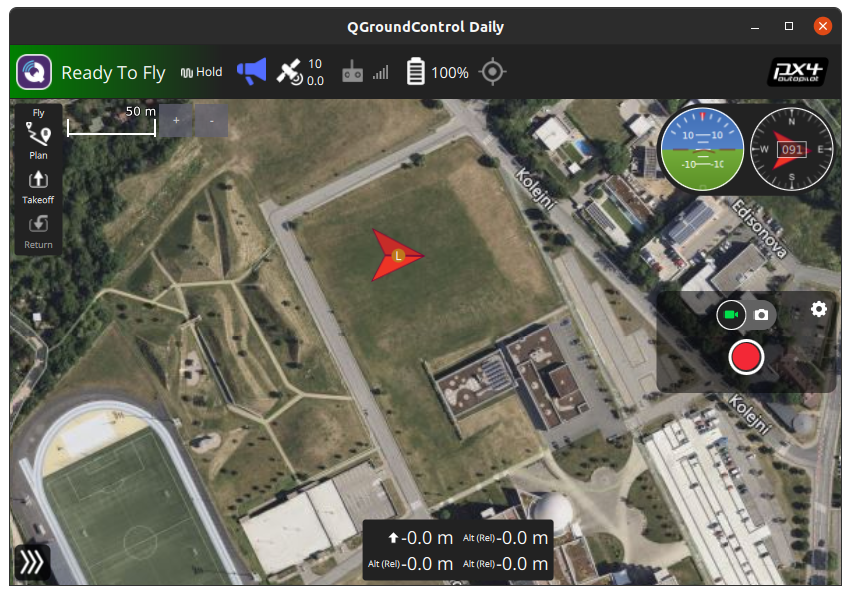
\includegraphics[scale=0.47]{obrazky/QG1}
    \end{center}
    \caption[Základní obrazovka QGroundControl]{Základní obrazovka QGroundControl.}
    \label{fig:QGC}
\end{figure}

Na základní obrazovce jsou zobrazeny stavové informace o dronu:

\begin{itemize}
    \item Relativní výška
    \item Azimut
    \item Orientace dronu (pitch, roll)
    \item RSSI (\textit{Received Signal Strength Indication})
    \item Počet připojených GPS satelitů
    \item Procento nabití akumulátoru
    \item Letový mód
\end{itemize}

\subsection{Nastavení konstrukce dronu}

Systém QGroundControl podporuje velké množství typů konstrukcí dronů, letadel, roverů a ponorek. Obrázek \ref{fig:QGC1} zobrazuje všechny podporované typy zařízení, které dokáže systém PX4 ovládat.

\begin{figure}[!ht]
    \begin{center}
        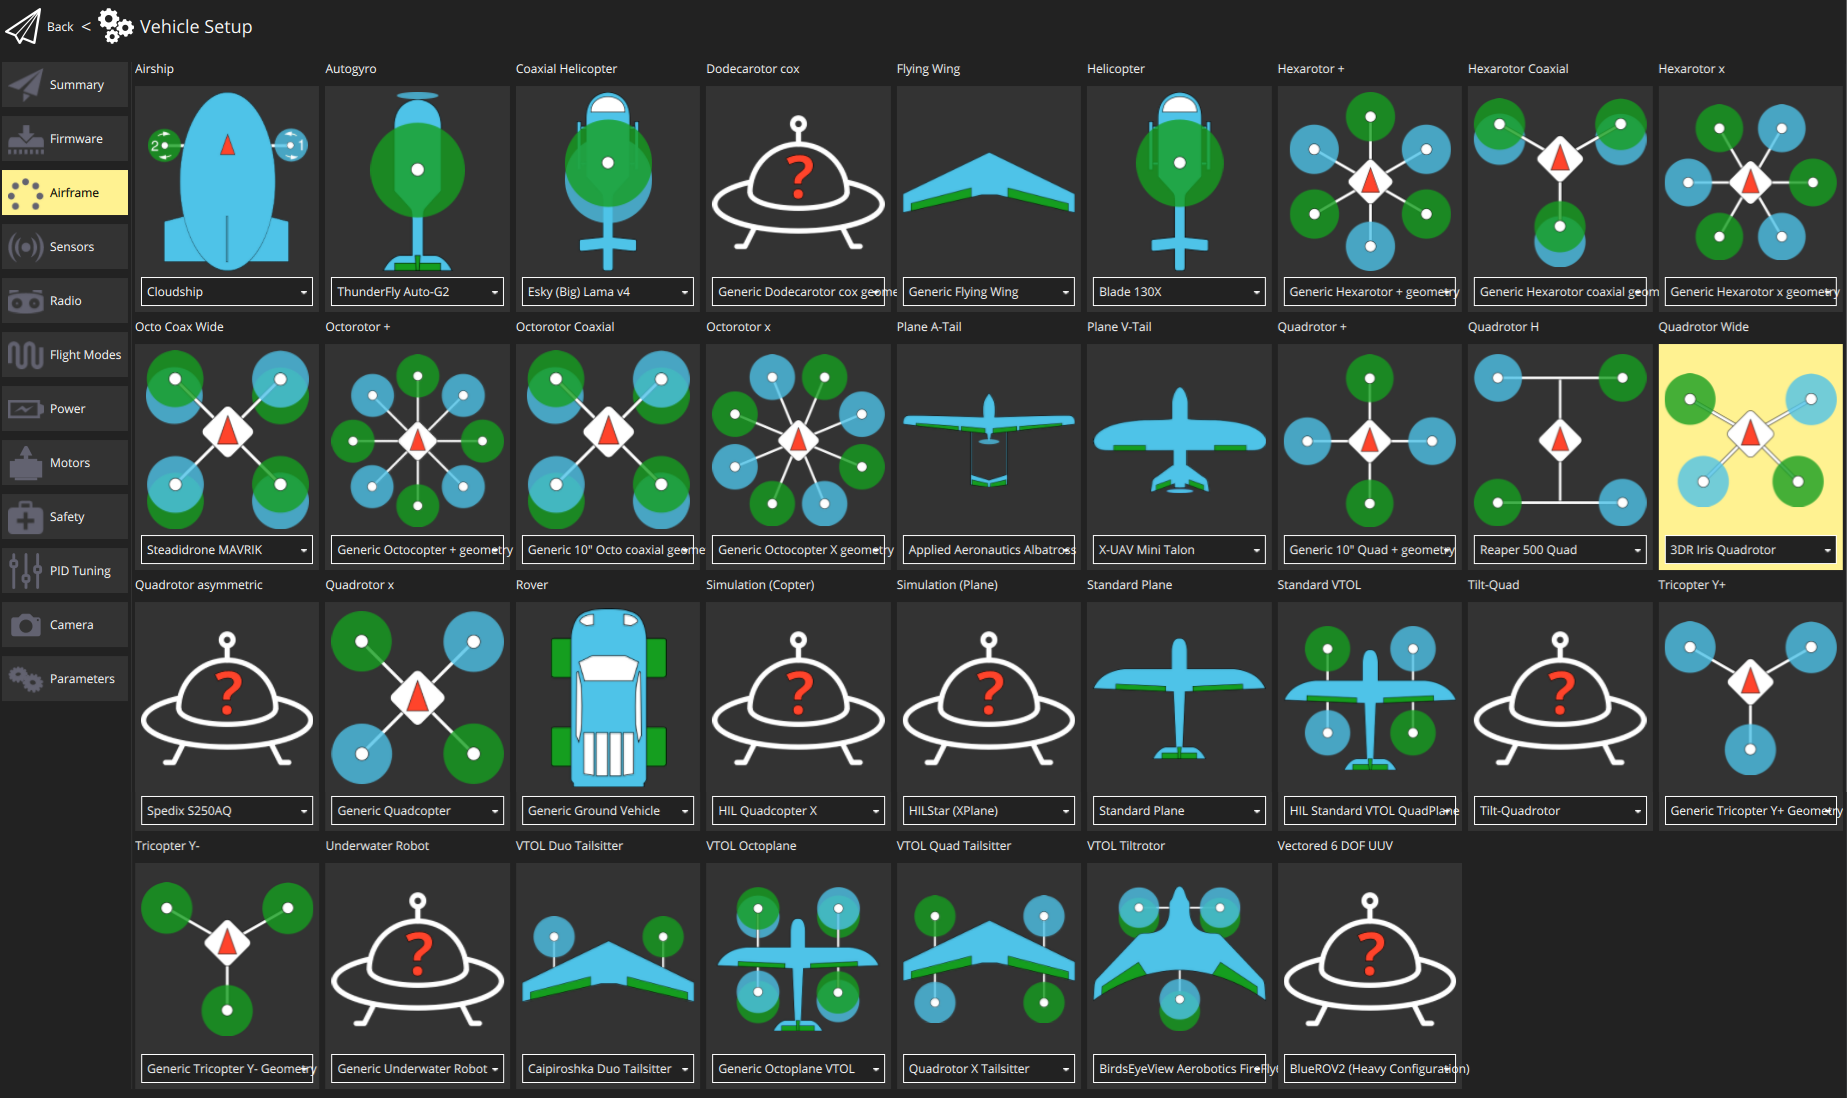
\includegraphics[scale=0.31]{obrazky/QG2}
    \end{center}
    \caption[Základní obrazovka QGroundControl]{Základní obrazovka QGroundControl.}
    \label{fig:QGC1}
\end{figure}

\subsection{Plánování bezpilotní mise}
\label{subs:planovani}

Software QGroundControl nabízí intuitivní plánování bezpilotních misí. Vlastní misi je možné naplánovat pomocí waypointů, nebo pomocí 3 přednastavených plánů pro bezpilotní mise: \cite{QGround2}

\begin{itemize}
    \item Průzkum prostředí
    \item Skenování koridoru
    \item Skenování konstrukcí
\end{itemize}

\subsubsection{Průzkum prostředí}

Pomocí tohoto plánu se vytvoří mřížkový letový vzor nad polygonální oblastí definovanou uživatelem. Oblast je možné definovat jako mnohoúhelník nebo kruh. Je zde taky možné nastavit mřížku přeletů, výšku nad povrchem jako absolutní, nebo relativní vůči terénu. Program umožňuje nastavení snímkování prostředí s podporou geotagging\footnote{Geotagging představuje přidávání geografických metadat k různým médiím jako jsou např.: obrázky.}. Obrázek \ref{fig:QGC2} zobrazuje nastavení autonomní mise s průzkumem prostředí.

\begin{figure}[!ht]
    \begin{center}
        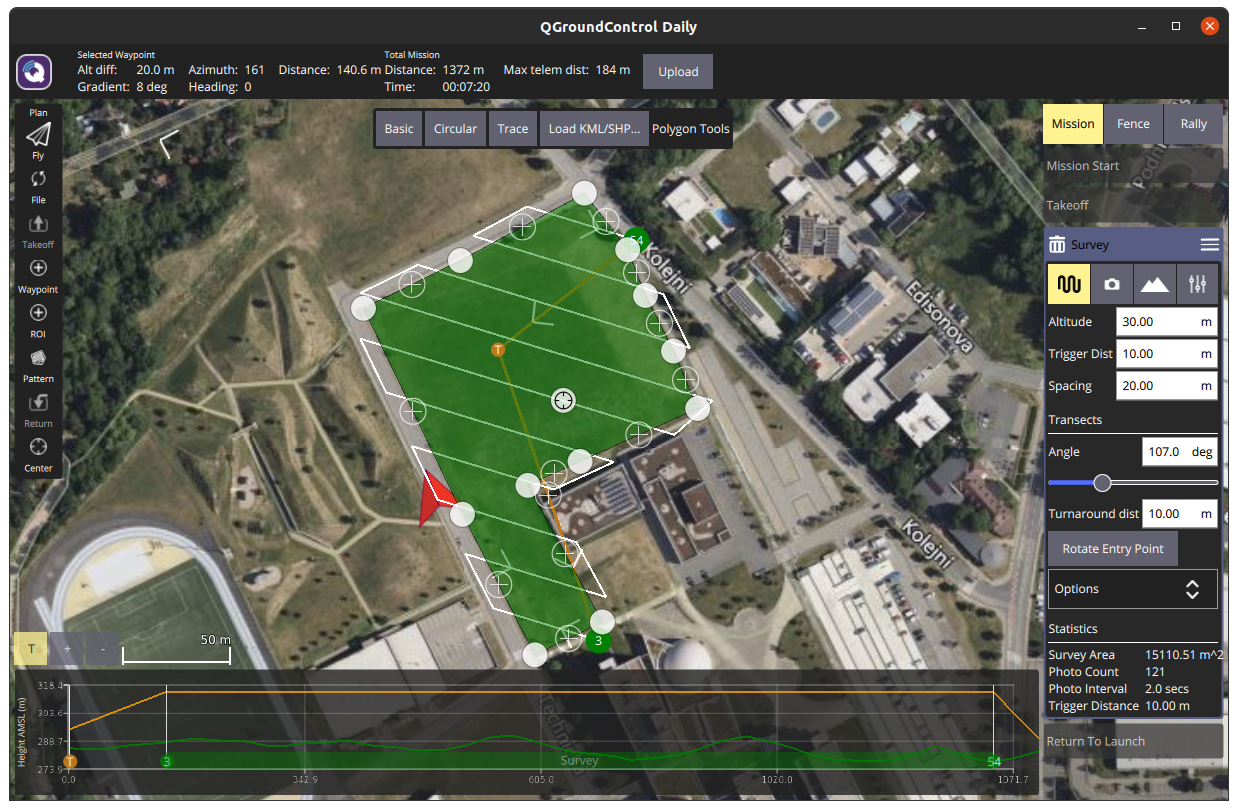
\includegraphics[scale=0.34]{obrazky/QGC3}
    \end{center}
    \caption[Nastavení bezpilotní mise pro průzkum prostředí]{Nastavení bezpilotní mise pro průzkum prostředí.}
    \label{fig:QGC2}
\end{figure}

\subsubsection{Skenování konstrukcí}

Pomocí plánu na skenování konstrukcí je možné naplánovat bezpilotní misi zaměřenou na snímkování svislých povrchů. Snímky se používají na vizuální kontrolu budov, nebo tvorbu 3D modelů konstrukcí. Obrys konstrukce je možné zadat jako mnohoúhelník nebo kruh. Dron bude oblétat celou budovu předem v nastavených výškách tak, aby kamera směřovala vždy na budovu. Po zadání konkrétní kamery, objektivu a rozlišení snímkování [cm/px] si program sám dopočítá vhodnou letovou vzdálenost od budovy a výšku jednotlivých letových vrstev. Na obrázku \ref{fig:QGC3} je zobrazeno nastavení autonomní mise pro skenování konstrukcí.

\begin{figure}[!ht]
    \begin{center}
        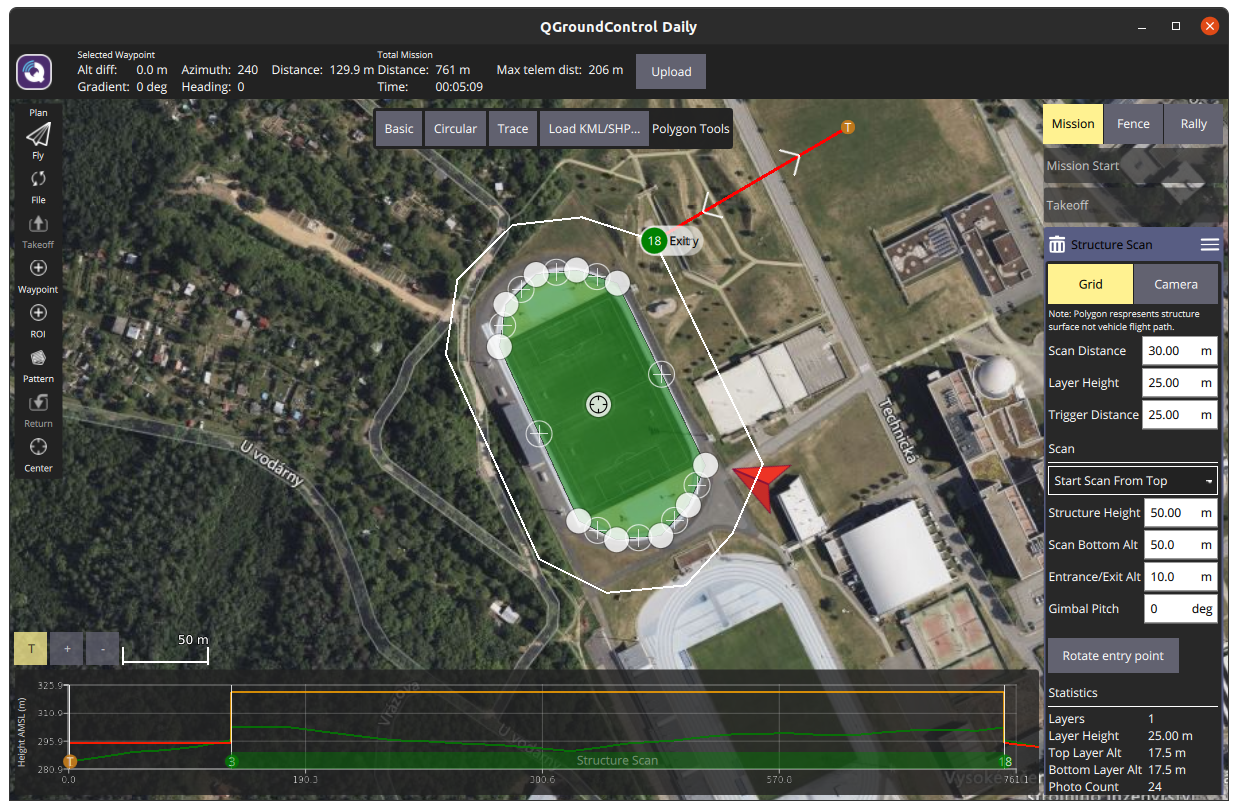
\includegraphics[scale=0.34]{obrazky/QGC5}
    \end{center}
    \caption[Nastavení bezpilotní mise pro skenování konstrukcí]{Nastavení bezpilotní mise pro skenování konstrukcí.}
    \label{fig:QGC3}
\end{figure}

\subsubsection{Skenování koridoru}

Letový plán pro skenování koridoru je vhodný pro sledování křivky (například pro průzkum silnice). Je možné si zde nastavit parametry letového vzoru jako jsou výška přeletu a hustota přeletů nad oblastí. Po zadání parametrů kamery a rozlišení snímkování [cm/px] si program sám dopočítá optimální letový vzor. Obrázek \ref{fig:QGC4} zobrazuje nastavení letového plánu pro skenování koridoru.

\begin{figure}[!ht]
    \begin{center}
        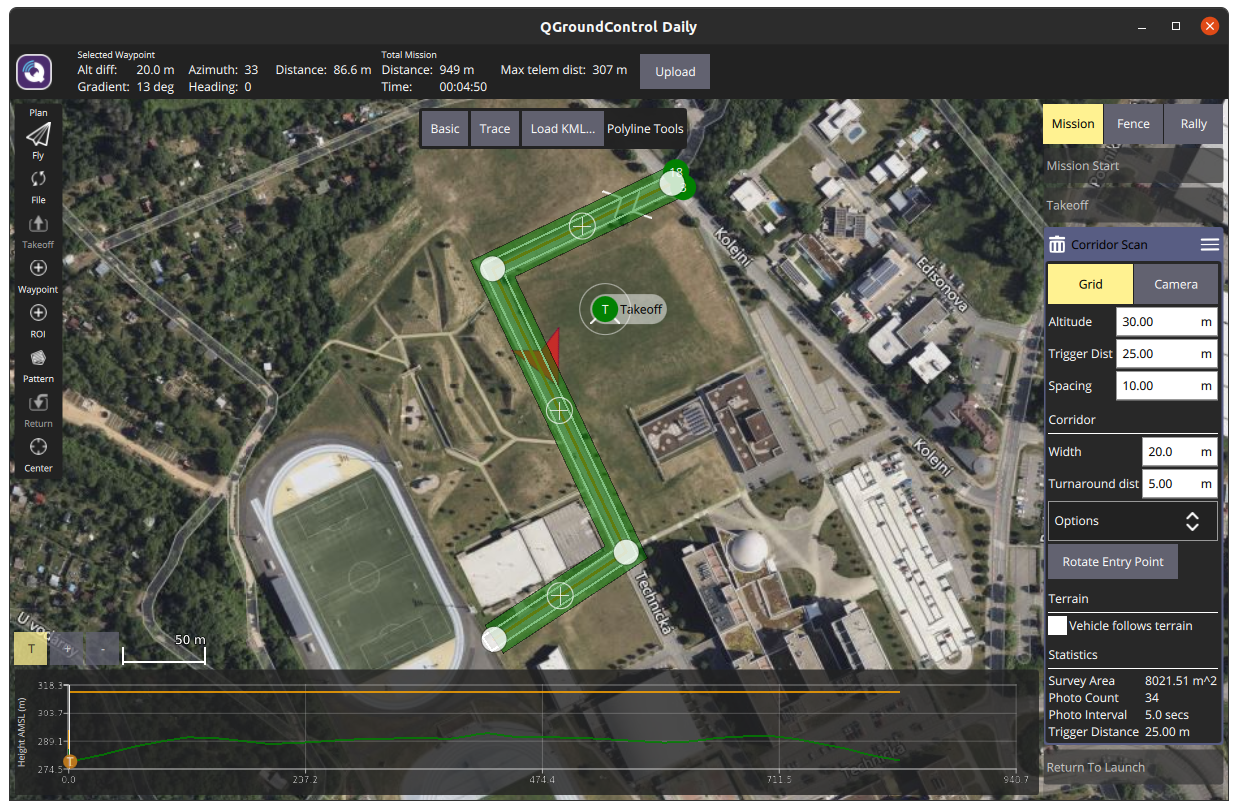
\includegraphics[scale=0.34]{obrazky/QGC4}
    \end{center}
    \caption[Nastavení bezpilotní mise pro skenování koridoru]{Nastavení bezpilotní mise pro skenování koridoru.}
    \label{fig:QGC4}
\end{figure}


\chapter{Simulace}

%%% Vložení souboru 'text/zaver' se závěrem
\chapter*{Závěr}
\phantomsection
\addcontentsline{toc}{chapter}{Závěr}

ZÁVER DOKONČIŤ

Tato semestrální práce se zabývala problematikou simulace misí bezpilotních letadel ve virtuálním prostředí ROS2/Gazebo. V první kapitole je popsána topologie dronu z pohledu řídícího systému. Zaobírá se jak řídící jednotkou pro nízkoúrovňové řízení dronu, tak palubním počítačem pro řízení složitých autonomních misí.

V další kapitole je popsán firmware pro řídící jednotku Pixhawk. Kapitola pojednává o architektuře firmware PX4 a o možnostech propojení a komunikace s ostatními periferiemi. Nedílnou součástí ekosystému PX4 je software QGroundControl pro vzdálenou kontrolu letu, plánování různých typů bezpilotních misí a nastavení dronu.

Důležitou částí práce je popis komunikace mezi ROS 2 a PX4 firmware přes Fast RTPS (\acs{DDS}) bridge. Práce rozebírá samotný \acs{DDS} (\acl{DDS}) middleware a jeho komunikační protokol \acs{RTPS} (\acl{RTPS}) pro kritické aplikace, základní vlastnosti \acs{DDS} a hlavně propojení mezi ROS 2 a \acs{DDS} komunikačním middleware.

Poslední kapitola popisuje simulaci ve virtuálním ekosystému PX4 - Gazebo - ROS 2. Shrnuje instalaci všech závislostí a postup sestavení simulačního prostředí (\textit{workspace}). Kapitola se zabývá tvořením a plánováním autonomní robotické mise, která je realizována pomocí ROS 2 balíčku a její testováním v simulačním prostředí. Cílem jednoduché autonomní mise je ovládat dron v tzv. \textit{offboard} módu pomocí ROS 2 balíčku. Podařilo se nám odsimulovat bezpilotní misi složenou z vzletu dronu, přeletu přes několik relativních souřadnic a následného přistání.



%%% Vložení souboru 'text/literatura' se seznamem zdrojů
% Pro sazbu seznamu literatury použijte jednu z následujících možností

%%%%%%%%%%%%%%%%%%%%%%%%%%%%%%%%%%%%%%%%%%%%%%%%%%%%%%%%%%%%%%%%%%%%%%%%%
%1) Seznam citací definovaný přímo pomocí prostředí literatura / thebibliography

\begin{thebibliography}{99}

    \bibitem{MRS}
MRS UAV System - open source platform for UAV research. \textit{Multi-robot Systems Group} [online]. Praha: Multi-robot Systems Group, c2022 [cit. 2022-01-01]. Dostupné z: \href{http://mrs.felk.cvut.cz/}{http://mrs.felk.cvut.cz/}

    \bibitem{PIX1}
The open standards for drone hardware. \textit{Pixhawk} [online]. San Francisco: Dronecode, 2018 [cit. 2022-01-01]. Dostupné z: \href{https://pixhawk.org/}{https://pixhawk.org/}

    \bibitem{PIX2}
Pixhawk 4. \textit{PX4} [online]. San Francisco: Dronecode, 2021 [cit. 2022-01-01]. Dostupné z: \href{https://docs.px4.io/master/en/flight\_controller/pixhawk4.html}{https://docs.px4.io/master/en/flight\_controller/pixhawk4.html}

	\bibitem{BSDlicense}
The 3-Clause BSD License: BSD-3-Clause. \textit{Open Source Initiative} [online]. West Hollywood: Open Source Initiative, 2014 [cit. 2021-11-17]. Dostupné z: \href{https://opensource.org/licenses/BSD-3-Clause}{https://opensource.org/licenses/BSD-3-Clause}

    \bibitem{PX4main}
PX4 Architectural Overview. \textit{PX4 Autopilot User Guide} [online]. San Francisco: Dronecode, 2021 [cit. 2021-12-19]. Dostupné z: \href{https://docs.px4.io/master/en/concept/architecture.html}{https://docs.px4.io/master/en/concept/architecture.html}

    \bibitem{PX4main2}
PX4 System Architecture. \textit{PX4 Autopilot User Guide} [online]. San Francisco: Dronecode, 2021 [cit. 2021-12-20]. Dostupné z: \href{https://docs.px4.io/master/en/concept/px4\_systems\_architecture.html}{https://docs.px4.io/master/en/concept/px4\_systems\_architecture.html}

	\bibitem{QGround}
QGroundControl. \textit{QGroundControl} [online]. San Francisco: Dronecode, 2019 [cit. 2021-11-24]. Dostupné z: \href{http://qgroundcontrol.com/}{http://qgroundcontrol.com/}

    \bibitem{QGround2}
QGroundControl User Guide. \textit{QGroundControl docs} [online]. San Francisco: Dronecode, 2021 [cit. 2021-12-21]. Dostupné z: \href{https://docs.qgroundcontrol.com/master/en/PlanView/Pattern.html}{https://docs.qgroundcontrol.com/master/en/PlanView/Pattern.html}

    \bibitem{ROS2DDS3}
ROS 2 middleware interface: Mapping between DDS and ROS concepts. \textit{ROS 2 Design} [online]. California: Open Source Robotics Foundation, 2017 [cit. 2021-12-21]. Dostupné z: \href{https://design.ros2.org/articles/ros\_middleware\_interface.html}{https://design.ros2.org/articles/ros\_middleware\_interface.html}

    \bibitem{UORB1}
UORB Messaging. \textit{PX4 Autopilot User Guide} [online]. San Francisco: Dronecode, 2021 [cit. 2021-12-21]. Dostupné z: \href{https://docs.px4.io/master/en/middleware/uorb.html}{https://docs.px4.io/master/en/middleware/uorb.html}

    \bibitem{UORBlist}
UORB Message Reference. \textit{PX4 Autopilot User Guide} [online]. San Francisco: Dronecode, 2021 [cit. 2021-12-24]. Dostupné z: \href{https://docs.px4.io/master/en/msg\_docs/}{https://docs.px4.io/master/en/msg\_docs/}

    \bibitem{UORB2}
RTPS/DDS Interface: PX4-Fast RTPS(DDS) Bridge. \textit{PX4 Autopilot User Guide} [online]. San Francisco: Dronecode, 2021 [cit. 2021-12-21]. Dostupné z: \href{https://docs.px4.io/master/en/middleware/micrortps.html}{https://docs.px4.io/master/en/middleware/micrortps.html}

    \bibitem{CDR}
EProsima Fast Buffers. \textit{EProsima the middleware experts} [online]. Madrid: eProsima, 2014 [cit. 2021-12-23]. Dostupné z: \href{https://www.eprosima.com/docs/fast-buffers/0.3.0/html/index.html}{https://www.eprosima.com/docs/fast-buffers/0.3.0/html/index.html}

    \bibitem{DDS_Standard}
The Real-time Publish-Subscribe Protocol (RTPS) DDS Interoperability Wire Protocol Specification. \textit{Object Management Group} [online]. Milford: OMG, c2021 [cit. 2021-11-25]. Dostupné z: \href{https://www.omg.org/spec/DDSI-RTPS/2.3}{https://www.omg.org/spec/DDSI-RTPS/2.3}
	
	\bibitem{DDS_Def}
Data Distribution Service (DDS). \textit{Object Management Group} [online]. Milford: OMG, 2018 [cit. 2021-11-25]. Dostupné z: \href{https://www.omg.org/omg-dds-portal/}{https://www.omg.org/omg-dds-portal/}

    \bibitem{DDS_Main}
What is DDS? \textit{DDS Foundation: Join DDS Foundation} [online]. Milford: DDS Foundation, c1997-2021 [cit. 2021-11-25]. Dostupné z: \href{https://www.dds-foundation.org/what-is-dds-3/}{https://www.dds-foundation.org/what-is-dds-3/}

    \bibitem{DDS_usage}
Why choose DDS?: Industry standards build on top of DDS. \textit{DDS Foundation: Join DDS Foundation} [online]. Milford: DDS Foundation, c1997-2021 [cit. 2021-11-25]. Dostupné z: \href{https://www.dds-foundation.org/why-choose-dds/}{https://www.dds-foundation.org/why-choose-dds/}

    \bibitem{DDS_PubSub}
Introduction to Publish/Subscribe. \textit{Real-Time Innovations: RTI | Inteligent, distributed and real world systems} [online]. Sunnyvale: RTI, c2020 [cit. 2021-11-28]. Dostupné z: \href{https://community.rti.com/static/documentation/connext-dds/6.0.1/doc/manuals/connext\_dds/getting\_started/cpp11/intro\_pubsub\_cpp.html}{https://community.rti.com/static/documentation/connext-dds/6.0.1/doc/manuals/connext\_cpp11/intro\_pubsub\_cpp.html}

    \bibitem{Eprosima}
RTPS Introduction: What is RTPS? \textit{EProsima: The Middleware experts} [online]. Madrid: eProsima, c2013-2021 [cit. 2021-11-29]. Dostupné z: \href{https://www.eprosima.com/index.php/resources-all/whitepapers/rtps}{https://www.eprosima.com/index.php/resources-all/whitepapers/rtps}

    \bibitem{ROS2DDS}
ROS on DDS: Technical Credibility of DDS. \textit{ROS 2 Design} [online]. California: Open Source Robotics Foundation, c2021 [cit. 2021-11-29]. Dostupné z: \href{https://design.ros2.org/articles/ros\_on\_dds.html}{https://design.ros2.org/articles/ros\_on\_dds.html}


    \bibitem{ROS2DDS2}
About different ROS 2 DDS/RTPS vendors: Supported RMW implementations. \textit{ROS 2 Documentation: Foxy} [online]. California: Open Robotics, c2021 [cit. 2021-12-09]. Dostupné z: \href{https://docs.ros.org/en/foxy/Concepts/About-Different-Middleware-Vendors.html}{https://docs.ros.org/en/foxy/Concepts/About-Different-Middleware-Vendors.html}

    \bibitem{SIM}
Simulation. \textit{PX4 Autopilot User Guide} [online]. San Francisco: Dronecode, 2021 [cit. 2021-12-28]. Dostupné z: \href{https://docs.px4.io/master/en/simulation/}{https://docs.px4.io/master/en/simulation/}

    \bibitem{GAZ}
\textit{Gazebo} [online]. California: Open Source Robotics Foundation, c2014 [cit. 2021-12-30]. Dostupné z: \href{http://gazebosim.org/}{http://gazebosim.org/}

    \bibitem{IGN}
THACKSTON, Allison. Ignition vs Gazebo. \textit{Allison Thackston} [online]. San Francisco: Thackston, c2014-2021 [cit. 2021-12-31]. Dostupné z: \href{https://www.allisonthackston.com/articles/ignition-vs-gazebo.html}{https://www.allisonthackston.com/articles/ignition-vs-gazebo.html}



% \bibitem{sr02/2009}
% 		VUT v~Brně:
%     \emph{Úprava, odevzdávání a zveřejňování vysokoškolských kva\-li\-fi\-kač\-ních prací na VUT v~Brně}\/ [online].
% 		Směrnice rektora č.\,2/2009.
% 		Brno: 2009, po\-sled\-ní aktualizace 24.\,3.\,2009 [cit.\,23.\,10.\,2015].
%     Dostupné z~URL:\\
%     <\url{https://www.vutbr.cz/uredni-deska/vnitrni-predpisy-a-dokumenty/smernice-rektora-f34920/}>.

% \bibitem{CSN_ISO_690-2011}
%     \emph{ČSN ISO 690 (01 0197) Informace a dokumentace -- Pravidla pro bibliografické odkazy a citace informačních zdrojů.}
%     40 stran. Praha: Český normalizační institut, 2011.

% \bibitem{CSN_ISO_7144-1997}
%     \emph{ČSN ISO 7144 (010161) Dokumentace -- Formální úprava disertací a podobných dokumentů.}
%     24 stran. Praha: Český normalizační institut, 1997.

% \bibitem{CSN_ISO_31-11}
%     \emph{ČSN ISO 31-11 Veličiny a jednotky -- část 11: Matematické znaky a značky používané ve fyzikálních vědách a v~technice.}
%     Praha: Český normalizační institut, 1999.

% \bibitem{BiernatovaSkupa2011:CSNISO690komentar}
%     BIERNÁTOVÁ, O., SKŮPA, J.:
%     \emph{Bibliografické odkazy a citace dokumentů dle ČSN ISO 690 (01 0197) platné od 1.\,dubna 2011}\/ [online].
%     2011, poslední aktualizace 2.\,9.\,2011 [cit. 19.\,10.\,2011].
%     Dostupné z~URL:
%     \(<\)\url{http://www.citace.com/CSN-ISO-690.pdf}\(>\)
% %    \(<\)\href{http://www.boldis.cz/citace/citace.html}{http://www.boldis.cz/citace/citace.html}\(>\).

% \bibitem{pravidla}
%     \emph{Pravidla českého pravopisu}.
%     Zpracoval kolektiv autorů. 1.\ vydání.
%     Olomouc: FIN PUB\-LISH\-ING, 1998. 575 s. ISBN 80-86002-40-3.

% \bibitem{Walter1999}
% 	WALTER, G.\,G.; SHEN, X.
% 	\emph{Wavelets and Other Orthogonal Systems}.
% 	2. vyd. Boca Raton: Chapman\,\&\,Hall/CRC, 2000. 392~s. ISBN 1-58488-227-1

% \bibitem{Svacina1999IEEE}
% 	SVAČINA, J.
% 	Dispersion Characteristics of Multilayered Slotlines -- a Simple Approach.
% 	\emph{IEEE Transactions on Microwave Theory and Techniques},
% 	1999, vol.\,47, no.\,9, s.\,1826--1829. ISSN 0018-9480.

% \bibitem{RajmicSysel2002}
%     RAJMIC, P.; SYSEL, P.
%     Wavelet Spectrum Thresholding Rules.
%     In \emph{Proceedings of the International Conference Research in Telecommunication Technology},
%     Žilina: Žilina University, 2002. s.\,60--63. ISBN 80-7100-991-1.

\end{thebibliography}


%%%%%%%%%%%%%%%%%%%%%%%%%%%%%%%%%%%%%%%%%%%%%%%%%%%%%%%%%%%%%%%%%%%%%%%%%
%%2) Seznam citací pomocí BibTeXu
%% Při použití je nutné v TeXnicCenter ve výstupním profilu aktivovat spouštění BibTeXu po překladu.
%% Definice stylu seznamu
%\bibliographystyle{unsrturl}
%% Pro českou sazbu lze použít styl czechiso.bst ze stránek
%% http://www.fit.vutbr.cz/~martinek/latex/czechiso.tar.gz
%%\bibliographystyle{czechiso}
%% Vložení souboru se seznamem citací
%\bibliography{text/literatura}
%
%% Následující příkaz je pouze pro ukázku sazby literatury při použití BibTeXu.
%% Způsobí citaci všech zdrojů v souboru literatura.bib, i když nejsou citovány v textu.
%\nocite{*}

%%% Vložení souboru 'text/zkratky' se seznam použitých symbolů, veličin a zkratek
\cleardoublepage
\chapter*{\listofabbrevname}
\phantomsection
\addcontentsline{toc}{chapter}{\listofabbrevname}

\begin{acronym}[KolikMista]

	\acro{IMU}
		[IMU]
		{Inertial Measurement Unit}
		
	\acro{SITL}
		[SITL]
		{Software In The Loop}
		
	\acro{HITL}
		[HITL]
		{Hardware In The Loop}
		
	\acro{CDR}
		[CDR]
		{Common Data Representation}
		
	\acro{API}
		[API]
		{Application programming interface}

    \acro{DDS}
		[DDS\textsuperscript \textregistered ]
		{Data-Distribution Service\textsuperscript \textregistered}
		
    \acro{RTPS}
		[RTPS]
		{Real Time Publish Subscribe protocol}
		
	\acro{DDSI}
	    [DDSI-RTPS\textsuperscript{\texttrademark} ]
	    {DDS Interoperability Wire Protocol\textsuperscript{\texttrademark}}
		
    \acro{QoS}
		[QoS]
		{Quality of Service}
		
	\acro{UDP}
		[UDP]
		{User datagram protocol}
		
	\acro{VTOL}
		[VTOL]
		{Vertical Take-Off and Landing}
		
	\acro{RTOS}
		[RTOS]
		{Real-Time Operating System}
		
	\acro{IDL}
		[IDL]
		{Interactive Data Language}
		
\end{acronym}


%%% Začátek příloh
%\appendix

%%% Vysázení seznamu příloh
% (vynechejte, pokud máte dvě nebo méně příloh)
%\listofappendices

%%% Vložení souboru 'text/prilohy' s přílohami
% Obvykle je přítomen alespoň popis co najdeme na přiloženém médiu
%\chapter{Přílohy}

\chapter{Obsah elektronické přílohy}
Elektronická příloha je často nedílnou součástí semestrální nebo závěrečné práce.
Vkládá se do informačního systému VUT v~Brně ve vhodném formátu (ZIP, PDF\,\dots).

Nezapomeňte uvést, co čtenář v~této příloze najde.
Je vhodné okomentovat obsah každého adresáře, specifikovat, který soubor obsahuje důležitá nastavení, který soubor je určen ke spuštění, uvést nastavení kompilátoru atd.
Také je dobře napsat, v~jaké verzi software byl kód testován (např.\ Matlab 2018b).
Pokud bylo cílem práce vytvořit hardwarové zařízení,
musí elektronická příloha obsahovat veškeré podklady pro výrobu (např.\ soubory s~návrhem DPS v~Eagle).

Pokud je souborů hodně a jsou organizovány ve více složkách, je možné pro výpis adresářové struktury použít balíček \href{https://www.ctan.org/pkg/dirtree}{\texttt{dirtree}}.

\bigskip

{\small
%
\dirtree{%.
.1 /\DTcomment{kořenový adresář přiloženého archivu}.
.2 logo\DTcomment{loga školy a fakulty}.
.3 BUT\_abbreviation\_color\_PANTONE\_EN.pdf.
.3 BUT\_color\_PANTONE\_EN.pdf.
.3 FEEC\_abbreviation\_color\_PANTONE\_EN.pdf.
.3 FEKT\_zkratka\_barevne\_PANTONE\_CZ.pdf.
.3 UTKO\_color\_PANTONE\_CZ.pdf.
.3 UTKO\_color\_PANTONE\_EN.pdf.
.3 VUT\_barevne\_PANTONE\_CZ.pdf.
.3 VUT\_symbol\_barevne\_PANTONE\_CZ.pdf.
.3 VUT\_zkratka\_barevne\_PANTONE\_CZ.pdf.
.2 obrazky\DTcomment{ostatní obrázky}.
.3 soucastky.png.
.3 spoje.png.
.3 ZlepseneWilsonovoZrcadloNPN.png.
.3 ZlepseneWilsonovoZrcadloPNP.png.
.2 pdf\DTcomment{pdf stránky generované informačním systémem}.
.3 student-desky.pdf.
.3 student-titulka.pdf.
.3 student-zadani.pdf.
.2 text\DTcomment{zdrojové textové soubory}.
.3 literatura.tex.
.3 prilohy.tex.
.3 reseni.tex.
.3 uvod.tex.
.3 vysledky.tex.
.3 zaver.tex.
.3 zkratky.tex.
%.2 navod-sablona\_FEKT.pdf\DTcomment{návod na používání šablony}.
.2 sablona-obhaj.tex\DTcomment{hlavní soubor pro sazbu prezentace k~obhajobě}.
%.2 readme.txt\DTcomment{soubor s~popisem obsahu CD}.
.2 sablona-prace.tex\DTcomment{hlavní soubor pro sazbu kvalifikační práce}.
.2 thesis.sty\DTcomment{balíček pro sazbu kvalifikačních prací}.
}
}


\end{document}